\documentclass[11pt,aspectratio=43]{beamer}
\usepackage{tikz}
\usetheme{Madrid}
\setbeamertemplate{navigation symbols}{}
\title{Constraint propagation: experiments and bounds}
\subtitle{Generated interaction study}
\author{Research group}
\date{}
\year=2026\month=11\day=5
\newcommand{\fuzzlayerA}[1]{\textit{#1}}
\newcommand{\fuzzterm}[1]{\fuzzlayerA{#1}}
\newcommand{\fuzzpair}[2]{\fuzzterm{#1}: #2}
\newcommand{\fuzzunit}{steps}
\let\fuzzoriginalunit\fuzzunit
\newcommand{\fuzzcoefficient}{1}
\newcommand{\fuzzscale}[2][\fuzzcoefficient]{#1\,#2}
\definecolor{fuzzpaint}{RGB}{255,0,255}
\definecolor{fuzzsecond}{RGB}{18,137,67}
\tikzset{fuzzvertex/.style={draw,rounded corners=1pt,fill=blue!10,inner sep=1pt,minimum width=.35cm,minimum height=.25cm}}
\begin{document}\begin{frame}[t]{Formatting boundary}
Before.\par
\begin{columns}[onlytextwidth,c]\begin{column}{.38\textwidth}Left text.\end{column}\begin{column}{0.58\textwidth}
\begin{enumerate}
\item<1-> \only<2->{{\scriptsize\color{teal}\raggedright
{\small\color{teal}\centering
\begin{columns}[onlytextwidth,T]
\begin{column}{0.38\textwidth}
\begin{tabular}{lrr}Method&Cost&Error\\\hline
Local0&0&22\\
Global1&11&4\\
Global2&26&17\\
\end{tabular}
\end{column}
\begin{column}{0.58\textwidth}
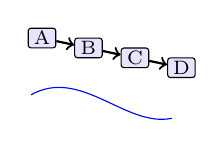
\begin{tikzpicture}[font=\scriptsize]
\begin{scope}[scale=0.8,rotate=-12]


\node[fuzzvertex] (g17n0) at (0.000,0) {A};
\node[fuzzvertex] (g17n1) at (0.754,0) {B};
\node[fuzzvertex] (g17n2) at (1.508,0) {C};
\node[fuzzvertex] (g17n3) at (2.262,0) {D};
\begin{scope}[xshift=.5pt,yshift=-.5pt]
\draw<1->[->,thick] (g17n0) -- (g17n1);
\draw<1->[->,thick] (g17n1) -- (g17n2);
\draw<1->[->,thick] (g17n2) -- (g17n3);
\draw[blue] (0,-.9) .. controls (0.679,-.3) and (1.583,-1.1) .. (2.262,-.8);
\end{scope}
\end{scope}
\end{tikzpicture}
\end{column}
\end{columns}\par}\par}}
\item<2-> \begin{flushright}
\begin{tabular}{lrr}Method&Cost&Error\\\hline
Global0&19&16\\
Cached1&16&15\\
Cached2&2&27\\
Global3&1&0\\
\end{tabular}
\end{flushright}
\end{enumerate}
\end{column}\end{columns}
Witness.\par\only<4>{}\end{frame}\end{document}
